%!TEX root = ../thesis.tex
\chapter{Experiments}

\label{ch:Experiments}

In this chapter I will show some experimental evidence of the effectiveness of the system which we have implemented.
Experiments are usually run against the competing systems Haxl\cite{Haxl:library:link}.
As mentioned in previous Chapters the code used for testing all systems in equal conditions is generated with our random code generator\cite{Goens-rand-code-graph}.
Additional boilerplate implementations for test data sources etc can be found in the \yauhau{} repository\cite{Yauhau:repository:link} for the \yauhau{} experiment code and for Haxl in the haxl-test-generated-graph\footnote{https://github.com/JustusAdam/haxl-test-generated-graph} repository.

\section{Functions}

This experiment shows the effectiveness of the round-detection algorithm on modularised code by generating program graphs which contains calls to algorithms.
Our experiment setup for this experiment operates on several graphs of constant depth (number of levels is constant).
We gradually increase the relative amount of algorithm calling nodes in the graph.
Additionally we run the series against multiple seeds to get an average result, hence fractional amounts of rounds.

\begin{figure}
    \includegraphics[width=\linewidth]{../Figures/func-experiment.eps}
    \caption{Number of rounds performed with functions enabled}
    \label{fig:experiment-functions}
\end{figure}

As is visible in the graph in Figure~\ref{fig:experiment-functions} our algorithm performs better than Haxl.
This is due to restrictions of using a runtime detection.
In Haxl the fetches inside a called function can only be inspected once all function parameters were provided and the term was bound to the monad.
Fetches which were independent from the function arguments therefore can still only be executed once the function received all input parameters
Since our algorithm operates on a dataflow graph and splices algorithms we can detect fetches which are independent from algorithm arguments and perform them before the algorithm would even be called.

\section{Smap}

This experiment show the quality of transformation for program graphs containing operations which map over a collection.
Our experiment setup for this experiment operates on several graphs of constant depth (number of levels is constant).
We gradually increase the relative amount of mapping operations in the graph.
Additionally we run the series against multiple seeds to get an average result.

In order to show that we in fact achieve the same performance with maps as Haxl does we run this experiment in two configurations.
For both configurations we operate on the same code graphs.
After the graphs have been generated we randomly select a number of nodes, with probabilities as listed on the x-axis in the plots.
We then change the type, and therefore the behaviour of those nodes, in two ways.

\begin{enumerate}
  \item The designated nodes become function invocations. Figure~\ref{fig:smap-experiment-primer}
        This is equivalent to attaching a small random subgraph to the node which is run once.
  \item The designated nodes become a an invocation of a mapping operation, \texttt{mapM} in Haxl and \texttt{smap} in \yauhau{}, over a function. Figure~\ref{fig:smap-experiment}
\end{enumerate}

For each node the invoked function and the mapped function are identical in both configurations, only the number of invocations changes.
In the first configuration, Figure~\ref{fig:smap-experiment-primer}, we can then see the flat performance advantage of \yauhau{} over Haxl independent from any \texttt{smap} or \texttt{mapM}.
We use this data to correct the data from the second experiment by this advantage to only get performance with respect to mapping operations.

In the second experiment, Figure~\ref{fig:smap-experiment}, we run the same graph as in the fist experiment, but here the nodes which used to be function invocations are now mappings.
The raw result data is then corrected by the difference from the previous experiment.
For each percentage of function/mapping nodes the difference in rounds created in the first experiment (Figure~\ref{fig:smap-experiment-primer}) is subtracted from the amount of rounds created for Haxl in the second experiment (Figure~\ref{fig:smap-experiment}).
This accounts for the flat benefit which \yauhau{} gains from the code style independence.
As is clearly visible in the plot in Figure~\ref{fig:smap-experiment} the performance of \yauhau{} and Haxl with respect to mapping operations is identical to that of Haxl.
Furthermore the performance with maps instead of function calls is actually identical to the performance achieved when using function calls (see ``No maps'' line in Figure~\ref{fig:smap-experiment}).
This shows that all fetches in mappings are indeed executed in parallel, as is intended.

\begin{figure}
    \includegraphics[width=\linewidth]{../Figures/smap-primer-experiment.eps}
    \caption{Rounds created with functions}
    \label{fig:smap-experiment-primer}
\end{figure}

\begin{figure}
    \includegraphics[width=\linewidth]{../Figures/smap-experiment.eps}
    \caption{Number of rounds performed with maps enabled}
    \label{fig:smap-experiment}
\end{figure}

\section{Conditionals}

As of late a fair amount of work has gone into understanding exactly how the different frameworks handle conditionals.
This is of particular interest because the code generator generates conditionals in a certain form and we would like to understand how that is translated and executed in each framework.

\subsection{Semantics of generated code}

Currently the code generator produces conditional code as seen in Figure~\ref{fig:generated-conditional-yauhau} for Yauhau and Figure~\ref{fig:generated-conditional-haxl} for Haxl.
From the Haxl example it is particularly obvious that values on both branches of the conditional are precomputed, that is the (monadic) operations necessary to compute both values are performed before the condition is being evaluated.
This has the consequence that any IO operation which is necessary to produce this value is performed before the condition for the \texttt{if} is evaluated and therefore might render the IO actions redundant if the value is not selected.
Of course the value might also be used in other, subsequent calculations, in which case precomputing is sensible.
In fact that is the reason why the graph serialisation in the code generator uses this particular style of code.
It does not inquire how many other nodes depend on the result of this calculation and hence obtains no knowledge of whether it is safe to move the computation onto the if branch itself.

\begin{figure}
\begin{minted}{Clojure}
(let [val1 (computation ...)
      val2 (computation ...)]
  (if condition val1 val2))
\end{minted}
\caption{Generated conditional code for Yauhau}
\label{fig:generated-conditional-yauhau}
\begin{minted}{Haskell}
do
  (val1, val2) <- (,) <$> computation ... <*> computation ...
  return $ if condition then val1 else val2
\end{minted}
\caption{Generated conditional code for Haxl}
\label{fig:generated-conditional-haxl}
\end{figure}

\begin{figure}
  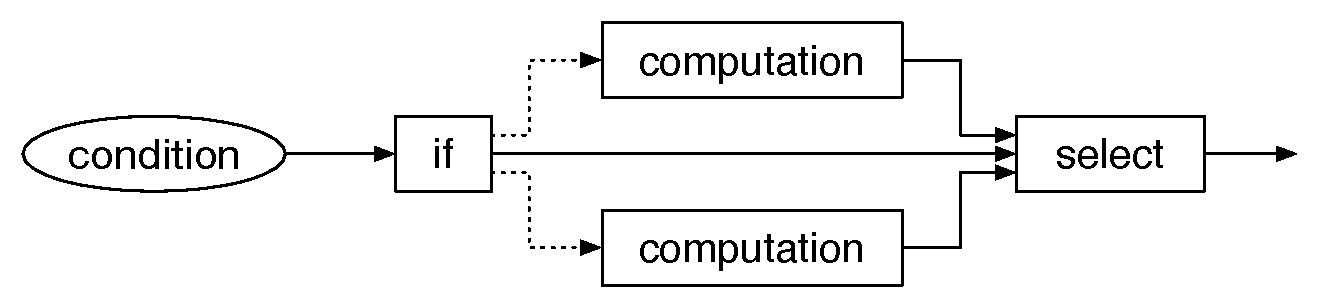
\includegraphics[width=\textwidth]{../Figures/if-hypothesised}
  \caption{Conditionals as hypothesised}
  \label{fig:if-graph-hypothesised}
  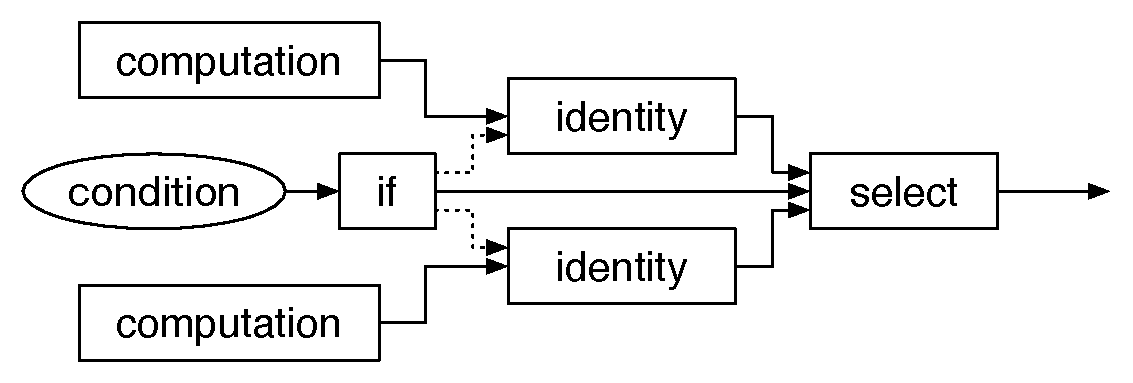
\includegraphics[width=\textwidth]{../Figures/if-in-reality}
  \caption{Conditionals actual}
  \label{fig:if-graph-actual}
\end{figure}

For a long time I suspected \yauhau{} and Ohua would handle this situation differently and \textbf{not} precompute the values, delay IO actions and only perform necessary calculations after evaluating the condition.
The reason we would come to this Hypothesis is because we thought operating on a dataflow graph would provide us with the necessary information and semantics by default.
However recently I discovered that, due to the way that we translates code into the dataflow graph, we do not in fact differ from Haxl in semantics.
As an example we will take the program from Figure~\ref{fig:generated-conditional-yauhau}.
We previously expected it to translate the program into a graph like the one in Figure~\ref{fig:if-graph-hypothesised}.
Here both computations are dependent on the \texttt{if} via a \textit{context arc} (dotted arrow) and therefore would be computed \textit{after} the condition had been evaluated.
The way in which Ohua would actually translate the program however would be to insert an operator called \texttt{value} on each of the if branches, which essentially wraps the bindings \texttt{val1} and \texttt{val2} respectively.
Additionally two \textit{context arcs} would be connected from the \texttt{if} to those \texttt{value} operators.
A visual representation of this can be seen in Figure~\ref{fig:if-graph-actual}.
At runtime, depending of the value of the condition, one of those \textit{context arcs} would be activated selecting the branch it is connected to, in this case the respective \texttt{value} operator.
In layman's terms the \texttt{if} selects one binding out of two at runtime, not one computation, as previously hypothesised.

We had also planned to show experiments later comparing the different semantics of \yauhau{} and Haxl when it comes to conditionals and discuss advantages and disadvantages of both.
Resulting from the recent unveilings however this has become redundant.
Since I hypothesised these two different semantics I put additional thought into advantages and disadvantages of precomputing potentially unused values and I want to use the following section to share my deliberations on the topic, backed by experimental evidence.


\subsection{Evaluation of precomputed conditional branches}

\label{sec:precomp-eval}

Let us assume that, in the system using Haxl or \yauhau{} computations are pure and the only stateful actions are the IO actions performed using the framework.
This view is of course not entirely consistent with reality, since nothing prevents you from doing effectful things in \yauhau{}, however in the domain where this system may be used it is a reasonable assumption to make for the purposes of the following deliberations.
Furthermore we may assume our fetches/reads to be \textit{pure} in so far as that they do not mutate the resource they request data from and serving a cached copy of a request is equivalent to actually performing the request.
How \yauhau{} deals with cases in which these assumptions do not hold is explained in detail in Chapter~\ref{ch:side-effects}.

If we assume the mentioned, lets call it \textit{near purity}, we can start to consider code reordering as an optimisation.
In particular reordering code around conditional statements is a possible code optimisation.
It turns out that, when performing batching transformations, like we do, moving requests out of, or into conditional branches has more intricate and interesting effects than it would in a regular program.

\subsubsection{New batching opportunities}

Consider a simple example (Figure~\ref{fig:requests-on-branches}) where we have a regular conditional statement and depending on the result of the computation one request.
Consider how this program would be batched.
The requests on the branches depend on the the evaluation of the condition and the condition depends on the data from \texttt{request0}, see also Figure~\ref{fig:requests-on-branches-graph}.
Fetch rounds are indicated by the blue, dashed rectangle.
As a result we would end up with two fetch rounds.
One for the request before the conditional and one for either the request from the true branch or the false branch.

\begin{figure}
\begin{minted}{Clojure}
(let [data1 (get-data request0 source1)]
  (if (computation data1)
    (get-data request1 source1)
    (get-data request2 source2)))
\end{minted}
\caption{Requests on branches}
\label{fig:requests-on-branches}
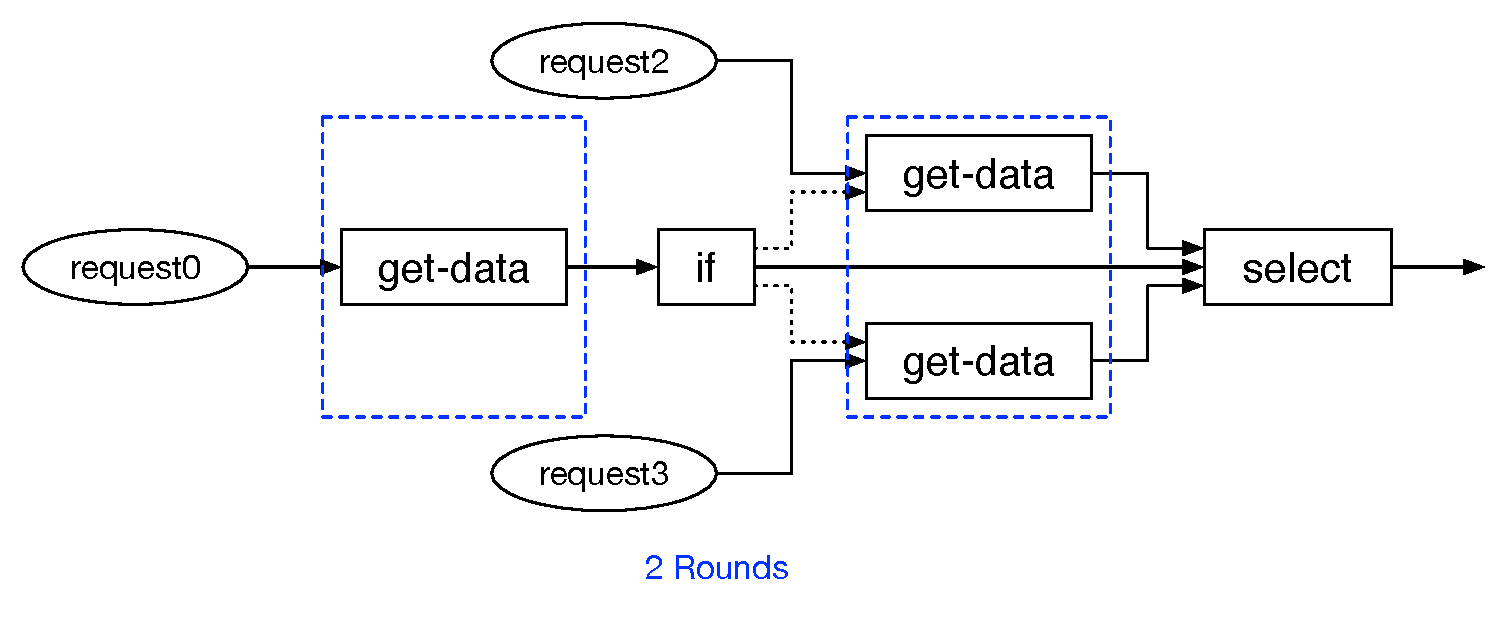
\includegraphics[width=\textwidth]{../Figures/requests-on-branches-graph}
\caption{Request on branches as graph}
\label{fig:requests-on-branches-graph}
\end{figure}

In \yauhau{} we generally operate under the assumption that IO actions are expensive.
The goal of our system is to do as few actual IO actions as possible.
In this case we see that we are performing two actions where we might only have to perform one action.
If we can, as previously mentioned, consider the fetches and computations as pure, we can rewrite the program to perform the conditional fetches \textbf{before} evaluating the condition (See Figure~\ref{fig:requests-precomputed}), which allows it to be batched with the first request, since the two fetches now do not depend on the condition anymore, See Figure~\ref{fig:requests-precomputed-graph}.
The round again indicated by the blue, dashed rectangle.
In particular if the fetch round before already includes a request to \texttt{source2} as well, then after our rewrite we get all the data from the entire second round for free.
For pure computations this will be semantically identical even though it performs redundant computation.

\begin{figure}
\begin{minted}{Clojure}
(let [data1 (get-data request0 source1)
      data2 (get-data request1 source1)
      data3 (get-data request2 source2)]
  (if (computation data1)
    data2
    data3))
\end{minted}
\caption{Requests precomputed}
\label{fig:requests-precomputed}
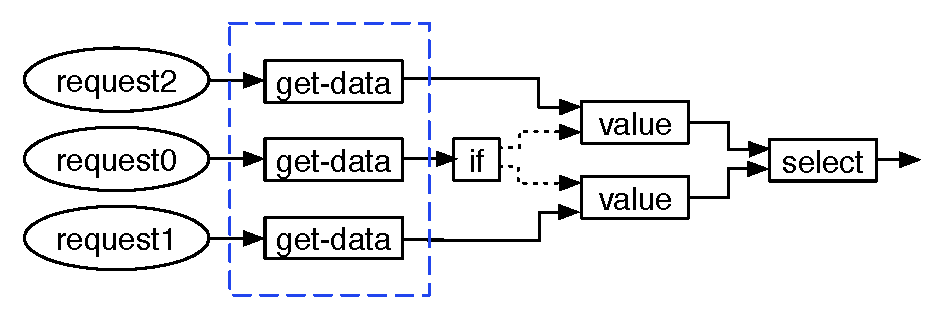
\includegraphics[width=\textwidth]{../Figures/requests-precomputed-graph}
\caption{Precomputed requests as graph}
\label{fig:requests-precomputed-graph}
\end{figure}

As also visible in Figure~\ref{fig:requests-precomputed} and \ref{fig:requests-precomputed-graph} this relocation of the data fetch results in more fetches being performed than in \ref{fig:requests-on-branches} we can see this in our experiment in Figure~\ref{fig:if-experiment-fetches}.

\begin{figure}
    \includegraphics[width=\linewidth]{../Figures/if-experiment-fetches.eps}
    \caption{Number of fetches performed}
    \label{fig:if-experiment-fetches}
\end{figure}

\begin{figure}
    \includegraphics[width=\linewidth]{../Figures/if-experiment.eps}
    \caption{Round difference}
    \label{fig:if-experiment}
\end{figure}

We have experimentally tested these hypotheses with code generated as described in Section~\ref{sec:extend-conditionals}.
What we found is that the amount of fetches in the precomputed version is significantly higher than in the inlined version, see Figure~\ref{fig:if-experiment-fetches}.
However in contrast to that the amount of performed rounds decreases as expected.
In Figure~\ref{fig:if-experiment} we see an average difference in the number of performed rounds, as well as a highest and lowest value for the number of rounds saved.
The precomputed version never performs more rounds than the inlined one and on average we save three rounds of IO when precomputing the branches, which means less execution time.
Figure~\ref{fig:if-experiment-prct} shows the average percentage of rounds which were saved my precomputing the branches with a minimum and maximum.

\begin{figure}
  \includegraphics[width=\textwidth]{../Figures/if-experiment-prct.eps}
  \caption{Round difference in percent}
  \label{fig:if-experiment-prct}
\end{figure}

\begin{figure}
    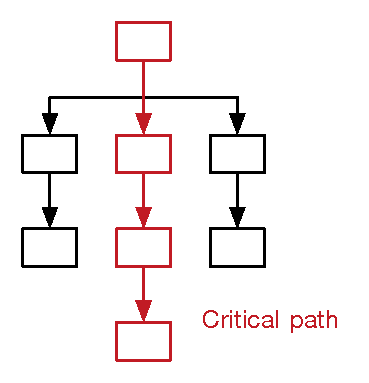
\includegraphics[width=.5\textwidth]{../Figures/critical-path}
    \caption{Critical path of fetches}
    \label{fig:critical-path}
\end{figure}

\subsubsection{Findings and explanation}

We can save up to 25\% of rounds and an average of about 15\% of rounds by precomputing conditional branches.
However these numbers were achieved in programs with a large number of conditional nodes.
Up to 95\% (of nodes with three children) were tagged and serialised as conditional nodes.
Considering this strong bias for conditionals the results seem pretty low.

The explanation for these low numbers seem to be that pulling fetches up into an earlier round only reduces the overall number of rounds if said fetch was part of the critical fetch path.
Like the critical path in a program we can construct a graph of data flow for only fetches where nodes are fetches and edges data reachability.
A visual representation of this can be seen in Figure~\ref{fig:critical-path}
The number of fetches along the longest path through this graph is the critical path with respects to fetches and marks a lower bound to the number of rounds we have to perform.
If the fetches we pulled from their branches were not part of the critical path pulling them up wont change the overall number of rounds at all, compare Figure~\ref{fig:rewrite-not-crit-path}, since there would have been a necessary later round which we cannot avoid performing and which could have incorporated the fetches from our branch.
Conversely if the fetches were part of the critical path, pulling them up reduces the length of the critical path, see Figure~\ref{fig:rewrite-crit-path}, ergo the optimal solution to minimal rounds decreases and our algorithm finds it.
Note that this is not limited to fetches on the critical fetch path of the original program but also to fetches on the new critical path resulting from a rewrite.

\begin{figure}
  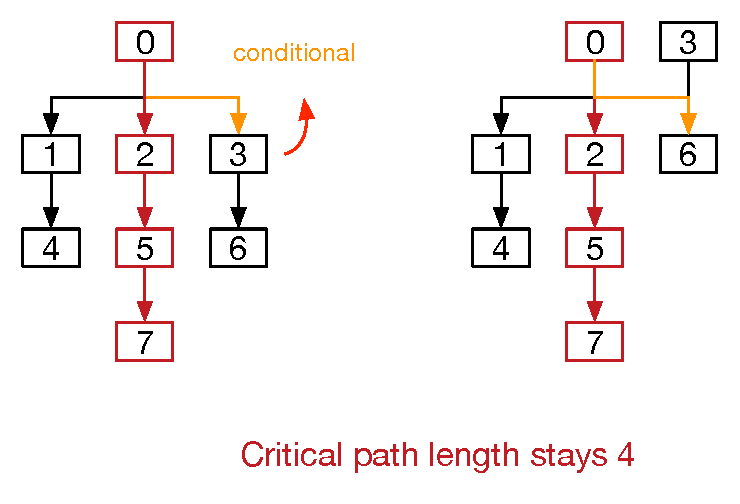
\includegraphics[width=\textwidth]{../Figures/rewrite-not-crit-path}
  \caption{Moving fetches not on the critical path}
  \label{fig:rewrite-not-crit-path}
\end{figure}

\begin{figure}
  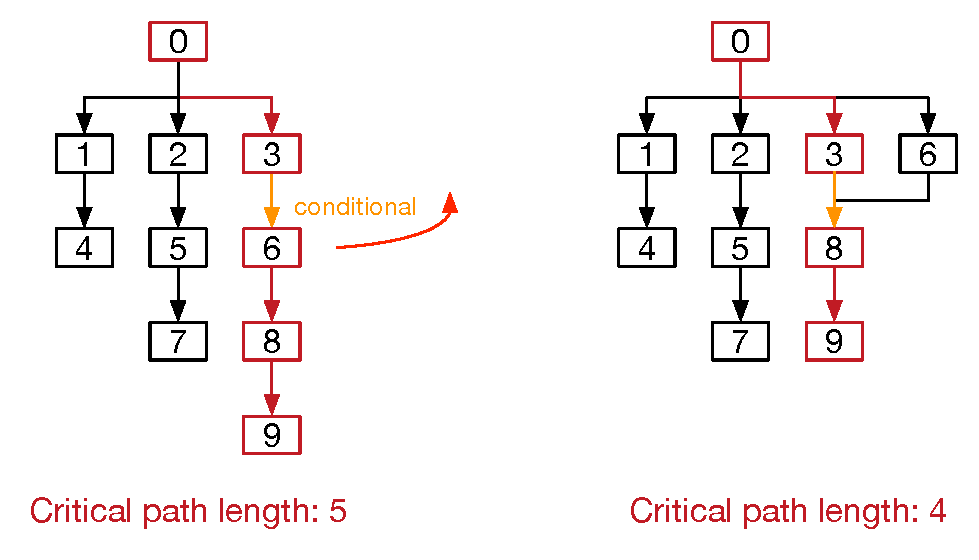
\includegraphics[width=\textwidth]{../Figures/rewrite-crit-path}
  \caption{Moving fetches on the critical path}
  \label{fig:rewrite-crit-path}
\end{figure}

\begin{figure}
  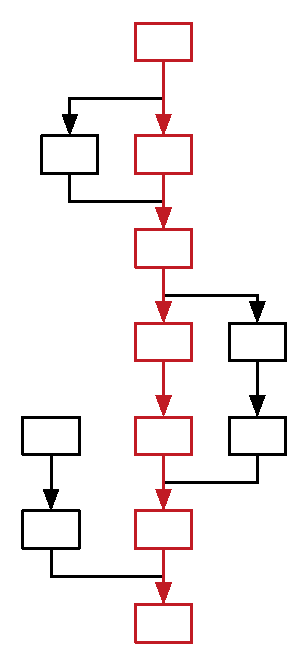
\includegraphics[width=.5\textwidth]{../Figures/dominant-critical-path}
  \caption{Fetch dataflow graph with dominant critical path}
  \label{fig:dominant-critical-path}
\end{figure}

\begin{figure}
  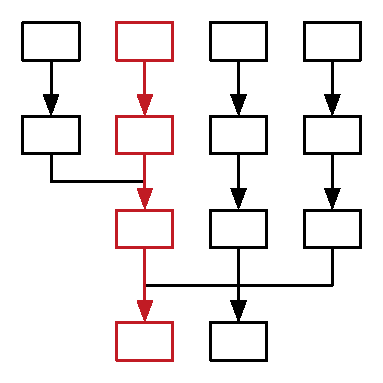
\includegraphics[width=.5\textwidth]{../Figures/non-dominant-critical-path}
  \caption{Fetch dataflow graph with no dominant critical path}
  \label{fig:non-dominant-critical-path}
\end{figure}

In these experiments I generate particularly narrow program graphs to create dominant critical paths, i.e. one long, interconnected path (Figure~\ref{fig:dominant-critical-path}) rather than several medium length paths (Figure~\ref{fig:non-dominant-critical-path}).

\subsubsection{Conclusion}

I have been able to show experimentally that precomputing conditional branches leads to new batching opportunities which \yauhau{} can take advantage of.
However I have also discovered that only some fetches actually benefit from this rewrite, namely those on the critical path.
In conclusion: considering the relatively small benefit even in program graphs with many \texttt{if}'s and dominant critical path the advantage from pulling subgraphs from conditional branches in a program can be considered negligible.
However it is useful for the programmer to be aware of these semantics and optionally perform these changes manually where applicable.
